
\chapter{Závěr}
V práci byly představeny NoSQL databáze jako nová databázová řešení, sloužící pro specifický druh využití, ale i jako náhrada relačních SQL databází. Byly představeny hlavní výhody NoSQL databází, jejich specifické vlastnosti a funkcionality. Práce popsala hlavní zástupce těchto databází a srovnala jejich možnosti použití v reálných webových aplikacích. Bylo provedeno porovnání NoSQL databáze MongoDB a SQL databáze MySQL, které se často používají ke stejnému účelu, tedy jako databáze pro webovou aplikaci, ukládájící objekty podle jejich typu. Klasické tabulky, známe z relačních databází v MongoDB představují kolekce. Tyto databáze byly nejprve srovnány teoreticky, podle jejich terminologie, syntaxe nebo reprezentace uložených dat. V praktické části byly provedeny výkonnostní testy těchto databází. Na základě těchto testů nebylo rozhodnuto, která databáze je opravdu lepší, byť v rychlosti zpracování většinou zvítězila NoSQL databáze MongoDB. 

NoSQL databáze neměly a ani nemají sloužit jako náhrada klasických relačních SQL databází, to ale nikdy nebyl ani jejich účel. První implementace vznikaly přímo na míru potřebám projektů, na kterých byly poté nasazeny, přímo na řešení určitých problémů, které vyvstaly. Hlavním důvodem jejich vzniku byla potřeba rychle a efektivně pracovat s obrovským množstvím dat. I proto byly průkopníky v této oblasti hlavně velké internetové firmy jako je Google nebo Facebook, které nedokázaly se svými obrovskými datovými objemy dobře pracovat pomocí tehdy dostupných technologií. Postupem času se našly další oblasti, kde  mohly NoSQL databáze najít své uplatnění. Rychlých key-value úložišť se začalo ve velkém využívat k ukládání velkého množství jednoduchých dat, velmi často jen například jedinečných idetifikátorů sezení pro každého přihlášeného uživatele. Dokumentově orientované databáze jsou vhodné pro strukturované ukládání nestejných dat. Jedná-li se o velké množství stejných dat, je výhodnější použít sloupcově orientovanou databázi. Grafové NoSQL databáze se zase velmi dobře hodí pro ukládání dat majících velké množství vazeb.

NoSQL databáze našly svá uplatnění, stejně jako ho našly klasické relační databáze a je jasné, že oba dva přístupy k ukládání a správě dat mohou existovat společně a je velmi těžké rozhodnout, který je ten „lepší“. Každý z těchto přístupů je má své výhody a nevýhody. MySQL přináší jednoduchý provoz, konzistenci dat a dotazovací jazyk SQL. MongoDB nabízí volnost podoby ukládaných dat a výborné možnosti škálování výkonu. Je na vývojářích, aby rozhodli která z těchto databází bude vhodnější pro použití v jejich aplikaci. Úkolem této práce bylo přinést srovnání dvou zcela odlišných databází, jejichž oblasti využití se překrývají.  

\section{Další směry výzkumu v oblasti}
Třetím testovacím prostředím, použitým v této práci, byl MongoDB databázový cluster. Ačkoli byl cluster ve většině testů pomalejší než MongoDB standalone server, a to z hlavně z důvodu virtualizace celého clusteru, bylo by zajímavé spustit provedené testy ještě na skutečném fyzickém clusteru. Potom by pravděpodobně MongoDB cluster zvítězil ve všech ohledech. Také by bylo možné do testů zařadit i MySQL Galera Cluster, tedy technologii pro distribuovaný běh relační databáze MySQL.

NoSQL databáze jsou velmi rozsáhlým tématem, existují desítky různých NoSQL databázových serverů, určených k obsluze různých typů dat. Zajímavým směrem vhodným pro další výzkum je tzv. \emph{Polygnot Persistance}. Tento koncept podle Martina Fowlera popisuje nasazení více databázových systémů zároveň pro různé druhy dat. Fowler udává, že pro každý typ dat je vhodné jiné prostředí, jiný jazyk a jiná databáze \cite{fowlerpp}. To znamená, že vedle sebe beží klasická relační databáze (na obrázku jako RDBMS), grafová databáze, dokumentově orientovaná databáze a další. Každá z těchto databází ukládá specifický typ dat, pro který je navržena nejlépe. Na obrázku níže jsou vidět různé databáze a jejich způsob využití ve fiktivní aplikaci. Je zde dobře vidět jak se mohou NoSQL databáze výborně doplňovat s relačními SQL databázemi.
\begin{figure}[h]
\begin{centering}
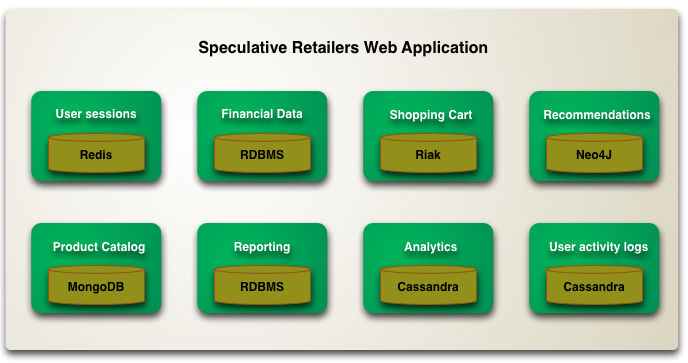
\includegraphics[scale=0.45]{obrazky/polygnot-persistance}
\par\end{centering}
\caption{Ukázka typů dat a jejich databází ve fiktivní aplikaci podle konceptu Polygnot Persistance \cite{fowlerpp}}.
\end{figure}